\title{ ProcessLunchOrders }
\author{Joe}
\date{\today}

\documentclass[12pt]{article}

\usepackage{tikz}
\usetikzlibrary{shapes,arrows}

\usepackage{listings}
\definecolor{mygreen}{rgb}{0,0.6,0}
\definecolor{mygray}{rgb}{0.5,0.5,0.5}
\definecolor{mymauve}{rgb}{0.58,0,0.82}

\usepackage{graphicx}
\graphicspath{ {Images} }

\lstset{numbers=left,commentstyle=\color{mygreen},keywordstyle=\color{blue}}


\begin{document}
\maketitle
\pagebreak

% Source Code
% ===========

\section{Source Code}

Source code for \textsf{processlunchorders.py}
\lstinputlisting[language=python,breaklines=true]{processlunchorders.py}

% Menu list imported from instructions
% \lstinputlisting[language=python,breaklines=true]{../menu.yaml}

\newpage

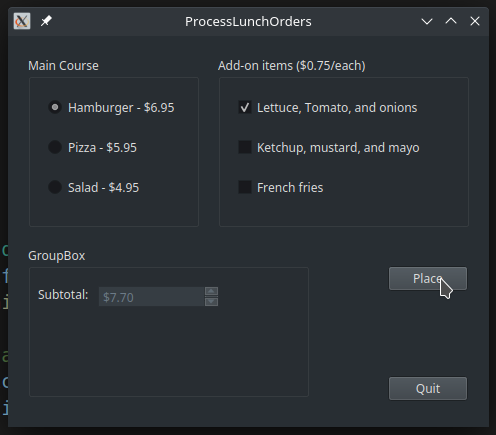
\includegraphics{Example1.png}
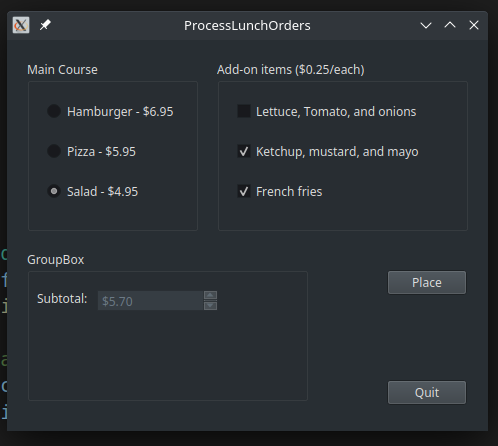
\includegraphics{Example2.png}

\newpage

\section{My Opinion}

I mean no disrespect I just wanted to vent here.

\vspace{2cm}

I am publicly vocal about my opion on \textbf{propriatary languages}. And while it is true that C\# has recently become open source i am still dissapointed
at every corner by the language.

Its not that I do not understand it, im fluent in both java and C\# and i mean no disrespect to you by submitting this in python. I will try and write
this assignment properly in C\# the moment I can, because i am behind.

I just wish to voice what i think about C\#, and my complaints, the overall workflow, the clunky package management. Its so bloated, unweildy, overwhelming.
Languages like Java, C\#, Pearl, these languages used in industry are not used productivly. I try and get by but Im simply not geared for this, at every
corner even just using winforms witch is \textbf{windows propriatary}, or the alternative gtk libraries. Its just so frustrating.

You cant even load a json without a build system, a dedicated windows packager or an IDE.

\newpage

Autogenerated using scripts by Joe and \LaTeX.

Please find the full source code and binaries included.

\end{document}
